% !TeX spellcheck = en_US
\documentclass[12pt, a4paper]{article}
\usepackage[scaled]{helvet}
\renewcommand\familydefault{\sfdefault}
\usepackage[T1]{fontenc}
\usepackage[margin=0.5in]{geometry}
\usepackage{float}
\usepackage{framed}
\usepackage{multicol}
\usepackage{amsmath}
\usepackage[framemethod=TikZ]{mdframed}
\usepackage{graphicx}
\usepackage{enumitem}
\setlist{nosep}

\newcounter{note}\setcounter{note}{0}
\renewcommand{\thenote}{\arabic{note}}
\newenvironment{note}[1]{
	\stepcounter{note}
	\ifstrempty{#1}{
		\mdfsetup{
			frametitle={
				\tikz[baseline=(current bounding box.east),outer sep=0pt]
				\node[anchor=east,rectangle,fill=blue!20]
				{\strut Note~\thenote};
			}
		}
	}{
		\mdfsetup{
			frametitle={
				\tikz[baseline=(current bounding box.east),outer sep=0pt]
				\node[anchor=east,rectangle,fill=blue!20]
				{\strut Note~\thenote:~#1};
			}
		}
	}
	\mdfsetup{innertopmargin=0pt,linecolor=blue!20,linewidth=2pt,topline=true,frametitleaboveskip=\dimexpr-\ht\strutbox\relax}
	\begin{mdframed}[]\relax
}{
	\end{mdframed}
}

\begin{document}
	\tableofcontents
	\vspace{2em}
	\textbf{Contributors:}
	\begin{itemize}
		\item Daniel Fitz (Sanchez)
	\end{itemize}
	
	\section{Sem Outline}
	\begin{table}[H]
		\begin{tabular}{ll}
			Week (dates) & Lecture\\
			1 & Computer Networks and the Internet\\
			2 & Principles of Nw Apps: HTTP, SMTP, DNS\\
			3 & Application Layer: P2P, CDN, Sockets\\
			4 & Networking at UQ\\
			5 & Transport Layer: UDP\\
			6 & Transport Layer: TCP\\
			7 & Network Layer: Data Plane\\
			8 & Network Layer: Control Place\\
			9 & Link Layer\\
			11 & Wireless and Mobile\\
			12 & Security\\
			13 & Multimedia
		\end{tabular}
		\centering
		\caption{Week Outline}
	\end{table}


\newpage
\begin{multicols*}{2}
	
	\section{Lecture 1}
	% !TeX spellcheck = en_US
% !TeX root = notes.tex
\begin{itemize}
	\item billions of connected computing devices
	\item transmission rate: \textbf{bandwidth}
	\item \textbf{Packet Switches:} Forward packets
	\begin{itemize}
		\item \textbf{routers} and \textbf{switches}
	\end{itemize}
	\item \textbf{Internet: ``network of networks''} (Interconnected ISPs)
	\item \textbf{Protocols} control sending, receiving (e.g. TCP, IP, HTTP, Skype, 802.11)
	\item \textbf{Internet standards}
	\begin{description}
		\item[RFC:] Request for comments
		\item[IETF:] Internet Engineering Task Force
	\end{description}
\end{itemize}

\subsection{Network Structure}
\begin{itemize}
	\item \textbf{Network Edge}
	\begin{itemize}
		\item hosts: clients and servers
		\item servers often in data centers
	\end{itemize}
	\item \textbf{Access networks, physical media:} wired, wireless communication links
	\item \textbf{network core:}
	\begin{itemize}
		\item interconnected routers
		\item network of networks
	\end{itemize}
\end{itemize}

\subsection{Access Network}
\subsubsection{Digital Subscriber Line (DSL)}
\begin{itemize}
	\item use \textbf{existing} telephone line to central office DSLAM
	\begin{itemize}
		\item data over DSL phone line goes to Internet
		\item voice over DSL phone line goes to telephone net
	\end{itemize}
	\item < 2.5 Mbps upstream transmission rate (typically < 1 Mbps)
	\item < 24 Mbps downstream transmission rate (typically < 10 Mbps)
\end{itemize}
\subsubsection{Cable Network}
\begin{leftbar}
	\textbf{frequency division multiplexing:} different channels transmitted in different frequency bands
\end{leftbar}
\begin{itemize}
	\item \textbf{HFC: hybrid fiber coax}
	\begin{itemize}
		\item asymmetric: up to 30Mbps downstream transmission rate, 2 Mbps upstream transmission rate
	\end{itemize}
	\item \textbf{network} of cable, fiber attaches homes to ISP router
	\begin{itemize}
		\item homes \textbf{share access network} to cable head-end
		\item unlike DSL, which has dedicated access to central office
	\end{itemize}
\end{itemize}
\textbf{wireless LANS:}
\begin{itemize}
	\item within building (30 meters)
	\item 802.11b/g/n (WiFi): 11,54,450 Mbps transmission rate
\end{itemize}
\textbf{wide-area wireless access:}
\begin{itemize}
	\item provided by telco (cellular) operator, 10's km
	\item between 1 and 10 Mbps
	\item 3G, 4G, LTE
\end{itemize}

\subsection{Sending}
\begin{itemize}
	\item takes application message
	\item breaks into smaller chunks, known as \textbf{packets}, of length \textbf{$L$} bits
	\item transmites packet into access network at \textbf{transmission rate $R$}
	\begin{itemize}
		\item link transmission rate, aka link \textbf{capacity, aka link bandwidth}
	\end{itemize}
\end{itemize}
\begin{note}{Packet Transmission Delay}
	\[
		\text{\parbox{2cm}{packet transmission delay}}=\text{\parbox{2cm}{time needed to transmit $L$-bit packet into link}}=\frac{L\text{ (bits)}}{R\text{ (bits/sec)}}
	\]
\end{note}

\subsection{Physical Media}
\begin{itemize}
	\item \textbf{bit:} propagates between transmitter/receiver pairs
	\item \textbf{physical link:} what lies between transmitter and receiver
	\item \textbf{guided media:} signals propagate in solid media (copper, fiber, coax)
	\item \textbf{unguided media:} signals propagate freely, e.g. radio
	\item \textbf{twisted pair (TP):} two insulated copper wires
	\begin{itemize}
		\item Category 5: 100 Mbps, 1 Gbps Ethernet
		\item Category 6: 10 Gbps
	\end{itemize}
\end{itemize}
\subsubsection{Coax}
\begin{itemize}
	\item two concentric copper conductors
	\item bidirectional
	\item broadband: multiple channels on cable, HFC
\end{itemize}
\subsubsection{Fiber Optic Cable}
\begin{itemize}
	\item glass fiber carrying light pulses, each pulse a bit
	\item high-speed operation: high-speed point-to-point transmission (e.g. 10's - 100's Gbps transmission rate)
	\item low error rate
	\begin{itemize}
		\item repeaters spaced far apart
		\item immune to electromagnetic noise
	\end{itemize}
\end{itemize}
\subsubsection{Radio}
\begin{itemize}
	\item signal carried in electromagnetic spectrum
	\item no physical "wire"
	\item bidirectional
	\item propagation environment effects:
	\begin{itemize}
		\item reflection
		\item obstruction by objects
		\item interference
	\end{itemize}
\end{itemize}
\textbf{Radio Link Types:}
\begin{itemize}
	\item \textbf{terrestrial microwave:} up to 45 Mbps channels
	\item \textbf{LAN} (e.g. WiFi) 54 Mbps
	\item \textbf{wide-area} (e.g. cellular) 4G cellular: \~ 10 Mbps
	\item \textbf{satellite}
	\begin{itemize}
		\item Kbps to 45 Mbps channel (or multiple smaller channels)
		\item 270 msec end-end delay
		\item geosynchronous versus low altitude
	\end{itemize}
\end{itemize}

\subsection{Packet-switching}
\subsubsection{Store-and-forward}
\begin{leftbar}
	$L$ bits per packet\\
	Source to destination: $R$ bps
\end{leftbar}
\begin{itemize}
	\item takes $\frac{L}{R}$ seconds to transmit (push out) $L$-bit packet into link at $R$ bps
	\item \textbf{store and forward:} entire packet must arrive at router before it can be transmitted on next link
\end{itemize}
\begin{note}{End-End delay}
	\[
		\text{delay} = 2\frac{L}{R}
	\]
	(assuming zero propagation delay)
\end{note}
\subsubsection{Packet switching versus circuit switching}
Is packet switching a ``slam dunk winner?''
\begin{itemize}
	\item great for bursty data (resource sharing, simpler, no call setup)
	\item excessive congestion possible: packet delay and loss (protocols needed for reliable data transfer, congestion control)
\end{itemize}

\subsection{Packet Loss}
\begin{figure}[H]
	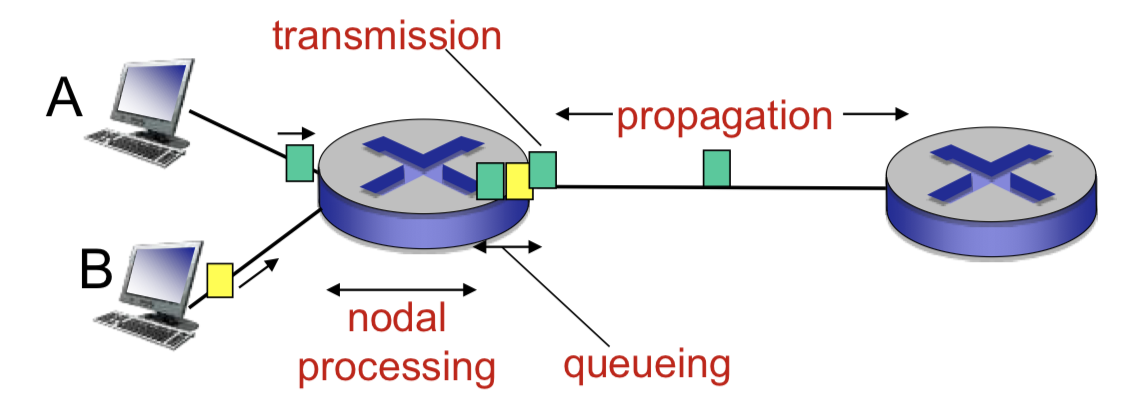
\includegraphics[width=8cm]{delay}
	\centering
	\caption{Packet Delay Algorithm Explanation}
\end{figure}
\begin{note}{Packet Delay Algorithm}
	\[ d_\text{nodal} = d_\text{proc} + d_\text{queue} + d_\text{trans} + d_\text{prop} \]
\end{note}
\subsubsection{Nodal Processing}
\[ d_\text{proc} \]
\begin{itemize}
	\item check bit errors
	\item determine output link
	\item typically < msec
\end{itemize}
\subsubsection{Queuing Delay}
\[ d_\text{queue} \]
\begin{itemize}
	\item time waiting at output link for transmission
	\item depends on congestion level of router
\end{itemize}
\subsubsection{Transmission Delay}
\[ d_\text{trans} \]
\begin{itemize}
	\item $L$: packet length (bits)
	\item $R$: link bandwidth(bps)
	\item $d_\text{trans} = \frac{L}{R}$
\end{itemize}
\subsubsection{Propagation Delay}
\[ d_\text{prop} \]
\begin{itemize}
	\item $d$: length of physical link
	\item $s$: propagation speed ($\approx2\times10^8$ m/sec)
	\item $d_\text{prop} = \frac{d}{s}$
\end{itemize}

\subsection{Throughput}
\begin{leftbar}
	Rate (bits/time unit) at which bits transferred between sender/receiver
\end{leftbar}
\begin{description}
	\item[Instantaneous:] rate at given point in time
	\item[Average:] rate over longer period of time
\end{description}
\begin{note}{Bottleneck Link}
	Link on end-end path that constrains end-end throughput
\end{note}

\subsection{Layering}
\subsubsection{Why Layering?}
Dealing with complex systems:
\begin{itemize}
	\item Explicit structure allows identification, relationship of complex system's pieces (layered \textbf{reference model} for discussion)
	\item Modularization eases maintenance, updating system
	\begin{itemize}
		\item change of implementation of layer's service transparent to rest of system
		\item e.g. change in gate procedure doesn't affect rest of system
	\end{itemize}
	\item layering considered harmful?
\end{itemize}
\subsubsection{Internet Protocol Stack}
\begin{description}
	\item[Application:] supporting network applications (FTP, SMTP, HTTP)
	\item[Transport:] process-process data transfer (TCP, UDP)
	\item[Network:] routing of datagrams from source to destination (IP, routing protocols)
	\item[Link:] data transfer between neighboring network elements (Ethernet, 802.111 (WiFi), PPP)
	\item[Physical:] bits ``on the wire''
\end{description}
\subsubsection{ISO/OSI Reference Model}
Internet stack ``missing'' these layers. These services, if needed, must be implemented in application.
\begin{description}
	\item[Application:]
	\item[Presentation:] allow applications to interpret meaning of data, e.g. encryption, compression, machine-specific conventions
	\item[Session:] synchronization, check-pointing, recovery of data exchange
	\item[Transport:]
	\item[Network:]
	\item[Link:]
	\item[Physical:]
\end{description}

\subsection{Security}
\begin{itemize}
	\item Malware can get in host from:
	\begin{description}
		\item[Virus:] self-replicating infection by receiving/executing object (e.g. e-mail attachment)
		\item[Worm:] self-replicating infection by passively receiving object that gets itself executed
	\end{description}
	\item \textbf{Spyware malware} can record keystrokes, web sites visited, upload info to collection site
	\item Infected host can be enrolled in \textbf{botnet}, used for spam. DDoS attacks
\end{itemize}
\subsubsection{DoS: Denial of Service}
\textbf{Denial of Service (DoS):} attackers make resources (server, bandwidth) unavailable to legitimate traffic by overwhelming resource with bogus traffic
\begin{enumerate}
	\item select target
	\item break into hosts around the network (botnet)
	\item send packets to target from compromised hosts
\end{enumerate}
\subsubsection{Sniffing}
\begin{itemize}
	\item broadcast media (shared Ethernet, wireless)
	\item promiscuous network interface reads/records all packets (e.g. including passwords) passing by
\end{itemize}
\subsubsection{IP Spoofing}
Send packet with false source address
	
	\section{Lecture 2}
	% !TeX spellcheck = en_US
% !TeX root = notes.tex
\subsection{Application Architectures}
\subsubsection{Client-Server}
\begin{description}
	\item[Server:] Always-on host, Permanent IP address
	\item[Clients:] Do not communicate directly with each other, May have dynamic IP addresses
\end{description}

\subsubsection{Peer-to-Peer (P2P)}
\begin{itemize}
	\item No always-on server
	\item Peers request service from other peers, provide service in return to other peers
	\item \textbf{Self Scalability} -- new peers bring new service capacity, as well as new service demands
	\item Pers are intermittently connected and change IP addresses
\end{itemize}

\begin{note}{App-layer protocol defines}
	\begin{itemize}
		\item \textbf{type of messages exchanged} -- e.g. request, response
		\item \textbf{message syntax} -- what fields in messages and how fields are delineated
		\item \textbf{message semantics} -- meaning of information in fields
		\item \textbf{rules} for when and how processes send and respond to messages
		\item \textbf{open protocols} -- defined in RFCs, allows for interoperability (e.g. HTTP, SMTP)
		\item \textbf{proprietary protocols} -- e.g. Skype
	\end{itemize}
\end{note}

\subsection{Transport Service is needed}
\begin{description}
	\item[Data Integrity:] Some programs need 100\% reliable data transfer (e.g. file transfer, web transactions), others can tolerate loss (e.g. audio)
	\item[Timing:] Some programs require low delay to be ``effective'' (e.g. online games)
	\item[Throughput:] Some programs require minimum amount of throughput to be ``effective'' (e.g. multimedia), some use whatever they have available (``elastic apps'')
	\item[Security:] Encryption, Data Integrity
\end{description}

\subsection{Transport Protocol Services}
\subsubsection{TCP}\label{sec:tcp}
\begin{description}
	\item[Reliable Transport] between sending and receiving process
	\item[Flow Control:] sender won't overwhelm receiver
	\item[Congestion Control:] throttle sender when network overloaded
	\item[Connection-Oriented:] setup required between client and server processes
	\item[Does Not Provide:] timing, minimum throughput guarantee, security
\end{description}

\subsubsection{UDP}\label{sec:udp}
\begin{description}
	\item[Unreliable Data Transfer] between sending and receiving process
	\item[Does Not Provide:] reliability, flow control, congestion control, timing, throughput guarantee, security, or connection setup
\end{description}

\subsubsection{Securing TCP}
\textbf{TCP and UDP}
\begin{itemize}
	\item no encryption
	\item cleartext passwords sent into socket traverse Internet in cleartext
\end{itemize}
\textbf{SSL}
\begin{itemize}
	\item provides encrypted TCP connection
	\item data integrity
	\item end-point authentication
\end{itemize}
\textbf{SSL is at app layer}
\begin{itemize}
	\item app use SSL libraries, that ``talk'' to TCP
\end{itemize}
\textbf{SSL socket API}
\begin{itemize}
	\item cleartext passwords sent into socket traverse Internet encrypted
\end{itemize}

\subsection{HTTP: Hypertext Transfer Protocol}\label{sec:http}
\begin{itemize}
	\item Web's application layer protocol
	\item client/server model. Client request website and server serves HTTP object in response
	\item Uses TCP
	\item HTTP is stateless. Server maintains no information about past client requests
	\item \textbf{non-persistent HTTP:} one object sent over one TCP connection, downloading multiple object required multiple connections
	\item \textbf{persistent HTTP:} multiple object sent over single TCP connection
\end{itemize}
Non-persistent HTTP issues:
\begin{itemize}
	\item requires 2 RTTs per object
	\item OS overhead for each TCP connection
	\item browsers often open parallel TCP connections to fetch referenced objects
\end{itemize}
Persistent HTTP:
\begin{itemize}
	\item server leaves connection open after sending response
	\item subsequent HTTP messages between same client/server sent over open connection
	\item client sends requests as soon as it encounters a referenced object
	\item as little as one RTT for all the referenced objects
\end{itemize}
\subsubsection{Method Types}
\textbf{HTTP/1.0:} GET, POST, HEAD (asks server to leave requested object out of response)\\
\textbf{HTTP/1.1:} GET, POST, HEAD, PUT (uploads file in entity body to path specified in URL field), DELETE (deletes file specified in the URL field)
\subsubsection{Response Codes}
\begin{description}
	\item[200 OK:] request succeeded, requested object later in this msg
	\item[301 Moved Permanently:] requested object moved, new location specified later in this msg
	\item[400 Bad Request:] request msg not understood by server
	\item[404 Not Found:] requested document not found on this server
	\item[505 HTTP Version Not Supported]
\end{description}

\subsection{Cookies}
Uses: authorization, shopping carts, recommendations, user session state (Web, email)

\subsection{Web Caches (proxy server)}
\begin{leftbar}
	\textbf{Goal:} satify client request without involving origin server
\end{leftbar}
\begin{itemize}
	\item Browsers requests object from cache, if in cache the object is sent back otherwise cache requests object from origin
	\item Cache acts as both client and server
	\item Reduce response time for client request
	\item Reduce traffic
\end{itemize}

\subsubsection{Conditional GET}
\begin{leftbar}
	\textbf{Goal:} don't send object if cache has up-to-date cached version (lower link usage)
\end{leftbar}
\begin{itemize}
	\item \textbf{Cache:} specify date of cached copy in HTTP request \texttt{If-modified-since: <date>}
	\item \textbf{Server:} response contains no object if cached copy is up-to-date: \texttt{HTTP/1.0 Not Modified}
\end{itemize}

\subsection{Electronic Mail: SMTP}\label{sec:smtp}
\textit{RFC 2821}
\begin{itemize}
	\item uses TCP to reliably transfer email message from client to server, port 25
	\item direct transfer: sending server to receiving server
	\item three phases of transfer: handshaking, transfer of messages, closure
	\item command/response interaction
	\item messages must be in 7-bit ASCII
	\item uses persistent connections
	\item requires message to be in 7-bit ASCII
	\item uses \texttt{CRLF.CRLF} to determine end of message
\end{itemize}
Difference to HTTP being, HTTP is server sending data, SMTP is client connection sending data\\
\begin{description}
	\item[SMTP:] protocol for exchanging email messages
	\item[RFC 822:] standard for text message format (To, From, Subject, Body)
\end{description}
\subsubsection{Mail Access Protocols}
\begin{leftbar}
	\textbf{SMTP:} delivery/storage to receiver's server
\end{leftbar}
\begin{description}
	\item[POP:] Post Office Protocol \textit{(RFC 1939)}: authorization, download
	\begin{itemize}
		\item POP3 is stateless across sessions
		\item Two main modes; download and delete, download and keep (allows multiple clients to read the same email)
	\end{itemize}
	\item[IMAP:] Internet Mail Access Protocol \textit{(RFC 1730)}: more features, including manipulation of stored message on server
	\begin{itemize}
		\item All messages stored on server
		\item Supports folders
		\item Keeps user state across sessions: names of folders and mappings between message IDs and folder name
	\end{itemize}
	\item[HTTP:] gmail, Hotmail, Yahoo, etc
\end{description}

\subsection{DNS: Domain Name System}\label{sec:dns}
\begin{itemize}
	\item Lookup between names (e.g. google.com) and IP addresses
	\item \textbf{Distributed Database} implemented in hierarchy of many \textbf{name servers}
	\item \textbf{Application-layer protocol:} hosts, name servers communicate to \textbf{resolve} names (address/name translation)
\end{itemize}
Why not centralize DNS? Single point of failure, traffic volume, doesn't scale
\subsubsection{DNS Services}
\begin{itemize}
	\item hostname to IP address translation
	\item host aliasing (canonical, alias names)
	\item mail server aliasing
	\item load distribution (many IP addresses correspond to one name)
\end{itemize}
\subsubsection{TLD, authoritative servers}
\textbf{top-level domain (TLD) servers:}
\begin{itemize}
	\item responsible for com, org, net, edu, aero, jos, io
	\item and top-level country domains au, uk, ca
	\item Network Solutions maintains servers for .com TLD
	\item Educause for .edu TLD
\end{itemize}
\textbf{Authoritative DNS servers:}
\begin{itemize}
	\item organization's own DNS server(s), providing authorative hostname to IP mappings for organization's named hosts
	\item can be maintained by organization or service provider
\end{itemize}
\subsubsection{Local DNS name server}
\begin{itemize}
	\item does not strictly belong to hierarchy
	\item each ISP (residential ISP, company, university) has one (also called ``default name server'')
	\item when host makes DNS query, query is sent to its local DNS server
	\begin{itemize}
		\item has local cache of recent name-to-address translation pairs (but may be out of date!)
		\item acts as proxy, forwards query into hierarchy
	\end{itemize}
\end{itemize}
\subsubsection{DNS Name Resolution}
\begin{description}
	\item[Iterated query:] contacted server replies with name of server to contact. So root dns sends the ip of the next dns server to contact
	\item[Recursive query:] puts burden of name resolution on contacted name server. So root dns server contacts the next levels down which contacts next level down.
\end{description}
\subsubsection{Caching}
Once (any) name server learns mapping, it \textbf{caches} mapping. Cache entries timeout (disappear) after some time (TTL). If name host changes IP address, the name servers might not update until TTLs expire.
\begin{leftbar}
	update/notify mechanisms proposed IETF standard RFC 2136
\end{leftbar}
\subsubsection{DNS Records}
\begin{note}{RR Format}
	\texttt{(name, value, type, ttl)}
\end{note}
\begin{description}
	\item[type=A] \texttt{name} is hostname, \texttt{value} is IP address
	\item[type=NS] \texttt{name} is domain (e.g. google.com), \texttt{value} is hostname of authoritative name server for this domain
	\item[type=CNAME] \texttt{name} is alias name for some ``canonical'' (the real) name (\texttt{www.ibm.com} is really \texttt{servereast.backup2.ibm.com}), \texttt{value} is canonical name
	\item[type=MX] \texttt{value} is name of mailserver associated with \texttt{name}
\end{description}
\subsubsection{Protocol}
Query and reply messages both follow same format
\begin{table}[H]
\centering
\caption{Protocol Layout}
\begin{tabular}{cc}
	\toprule
	2 bytes & 2 bytes \\
	\midrule
	identification & flags\\
	\# questions & \# answer RRs\\
	\# authority RRs & \# additional RRs\\
	\multicolumn{2}{c}{questions (variable \# of questions)}\\
	\multicolumn{2}{c}{answers (variable \# of RRs)}\\
	\multicolumn{2}{c}{authority (variable \# of RRs)}\\
	\multicolumn{2}{c}{additional info (variable \# of RRs)}\\
	\bottomrule
\end{tabular}
\end{table}
\subsubsection{Attacking DNS}
\textbf{DDoS attacks}
\begin{itemize}
	\item bombard root servers with traffic. Not successful to date, traffic filtering, local DNS servers cache protecting root DNS
	\item bombard TLD server. Potentially more dangerous
\end{itemize}
\textbf{Redirect Attacks}
\begin{itemize}
	\item man-in-middle (Intercept queries)
	\item DNS Poisoning (Send bogus relies to DNS server, which caches)
\end{itemize}
\textbf{Exploit DNS for DDoS}
\begin{itemize}
	\item send queries with spoofed source address: target IP
	\item requires amplification
\end{itemize}
	
	\newpage
	\section{Acronyms}
	% !TeX spellcheck = en_US
% !TeX root = notes.tex

\begin{description}
	\item[IP:] Internet Protocol
	\item[TCP:] 
	\item[UDP:] 
	\item[HTTP:] Hypertext Transfer Protocol
	\item[SMTP:] Simple Mail Transfer Protocol
	\item[RDP:]	Remote Desktop Protocol
	\item[VOIP:] Voice over IP
	\item[RTT:]
	\item[POP:] Post Office Protocol
	\item[IMAP:] Internet Mail Access Procotol
	\item[DNS:] Domain Name System
	\item[SSN:]
	\item[TLD:] Top-level Domain
	\item[TTL:] Time To Live
	\item[RR:] Resource Records
	\item[DDoS:]
	\item[CBR:] Constant bit rate
	\item[VBR:] Variable bit rate
	\item[ABR:]
	\item[UBR:]
	\item[DASH:] Dynamic, Adaptive Streaming over HTTP
	\item[CDN:] Content Distribution Networks
	\item[RDT:] Reliable Data Transfer
	\item[MSS:]
	\item[ECN:] Explicit Congestion Notification
	\item[ECE:]
	\item[SDN:] Software-defined networking
	\item[TCAMs:] Ternary Content Addressable Memories
	\item[HOL:] Head-of-the-Line
	\item[FIFO:] First in first out
	\item[RR:] Round Robin
	\item[WFQ:] Weighted Fair Queuing
	\item[CIDR:] Classless InterDomain Routing
	\item[DHCP:] Dynamic Host Configuration Protocol
	\item[ICANN:] Internet Corporation for Assigned Names and Numbers
	\item[NAT:] Network Address Translation
	\item[QoS:]
	\item[OSPF:]
	\item[ODL:]
	\item[ONOS:]
	\item[ICMP:] Internet Control Message Protocol
	\item[SNMP:]
	\item[CA:] Control Agent
	\item[DV:] Distance Vector
	\item[B-F:] Bellman-Ford
	\item[LS:] Link State
	\item[AS:] Autonomous Systems
	\item[IGP:] Interior Gateway Protocols
	\item[RIP:] Routing Information Protocol
	\item[OSPF:] Open Shortest Path First
	\item[IGRP:] Interior Gateway Routing Protocol
	\item[ToS:]
	\item[MOSPF:] Multicast OSPF
	\item[BGP:] Border Gateway Protocol
	\item[SDN:] Software Defined Networking
	\item[SNMP:]
	\item[ODL:] OpenDaylight
	\item[SAL:] Service Abstraction Layer
	\item[OVSDB:]
	\item[MIB:] Management Information Base
\end{description}


\end{multicols*}	
\end{document}